\textbf{ID:} UC10 (Create Post) \\
\textbf{Scope:} CS Automated Information Timeline \\
\textbf{Level:} User Goal \\
\textbf{Stakeholders and Interests:}
\begin{itemize}
    \item Faculty: A person who works for the university and is interested in gaining visibility of this post and/or event.
    \item Admin/Reviewer: A person who works for the university and approves and/or removes posts and/or event from the system.
\end{itemize}
\textbf{Preconditions:}
\begin{itemize}
    \item Faculty, f, has been identified and authenticated.
\end{itemize}
\textbf{Postconditions:}
\begin{itemize}
    \item Post, p, was created.
    \item p.status was set to “Pending”.
    \item p.createdBy was set to Faculty f.
    \item Post, p, was persisted.
    \item Notification, n, was created.
    \item n.post was set to Post p.
    \item Notification, n, was persisted.
\end{itemize}
\textbf{Main Success Scenario:}
\begin{enumerate}
    \item Faculty writes the post using the post creation tool.
    \item The post title is written by the faculty user.
    \item The post body is written by the faculty user.
    \item Faculty reviews the post draft.
    \item Faculty submits the post to the system.
    \item A post id is generated by the system.
    \item A timestamp is generated by the system.
    \item The user id of the faculty user is attached to the post object.
    \item The system assigns the status of the post to the proposed state.
    \item The system generates a notification object.
    \item The post object is attached to the notification object.
    \item The post object is persisted.
    \item The notification object is persisted.
    \item The system returns the persisted post object to the faculty user.
\end{enumerate}
\textbf{Extensions:} \\\relax
*.a. Anytime the system does not respond.
\begin{enumerate}
    \item Faculty will notify the Admin/Reviewer.
    \item Admin/Reviewer will restart the system.
    \item Faculty will recreate and submit the post.
\end{enumerate}
5.a. Anytime the system does not respond.
\begin{enumerate}
    \item The system will return an error message to the faculty user.
    \item The faculty user will resubmit the post.
\end{enumerate}
6.a. If the post is not persisted.
\begin{enumerate}
    \item The system will return an error message to the faculty user.
    \item The faculty user will reattempt the submission of the post.
\end{enumerate}
\textbf{Special Requirements:} None \\
\textbf{Technology and Data Variations List: }
\begin{enumerate}
    \item Date will be of the format “yyyy-MM-ddTHH:mm:ss”.
    \item Id will be of the format of a universally unique identifier, UUID.
\end{enumerate}
\textbf{Frequency of Occurrence:} Could be nearly continuous. \\

\begin{figure}[H]
    \centering
    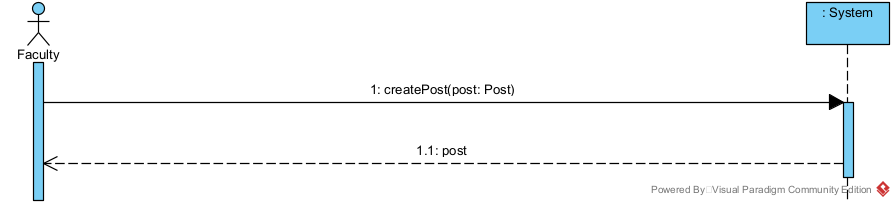
\includegraphics[width=0.8\textwidth]{images/SSD-UC10-CreatePost.png}
    \centering
    \caption{System Sequence Diagram: Create Post}
\end{figure}

\textbf{Operation:} createPost(post: Post) \\
\textbf{Cross References:} UC10 (Create Post) \\
\textbf{Preconditions:}
\begin{itemize}
    \item Faculty, f, has been identified and authenticated.
\end{itemize}
\textbf{Postconditions:}
\begin{itemize}
    \item Post, p, was created.
    \item p.status was set to “Pending”.
    \item p.createdBy was set to Faculty f.
    \item Post, p, was persisted.
    \item Notification, n, was created.
    \item n.post was set to Post p.
    \item Notification, n, was persisted.
\end{itemize}